\chapter{Aqu\'i va el t\'itulo del Cap\'itulo 1}

\noindent Las referencias se realizan, por ejemplo, de la siguiente manera: ... (cf. \cite{Abraham-Marsden-Ratiu:MTAA}). Cuando agregas una referencia nueva debes compilar \texttt{pdflatex} dos veces, luego \texttt{bibtex} y nuevamente \texttt{pdflatex} dos veces, esto actualiza las referencias a la bibliograf\'ia.
\bigskip

Puedes agregar im\'agenes:

\begin{figure}[h]
\begin{center}
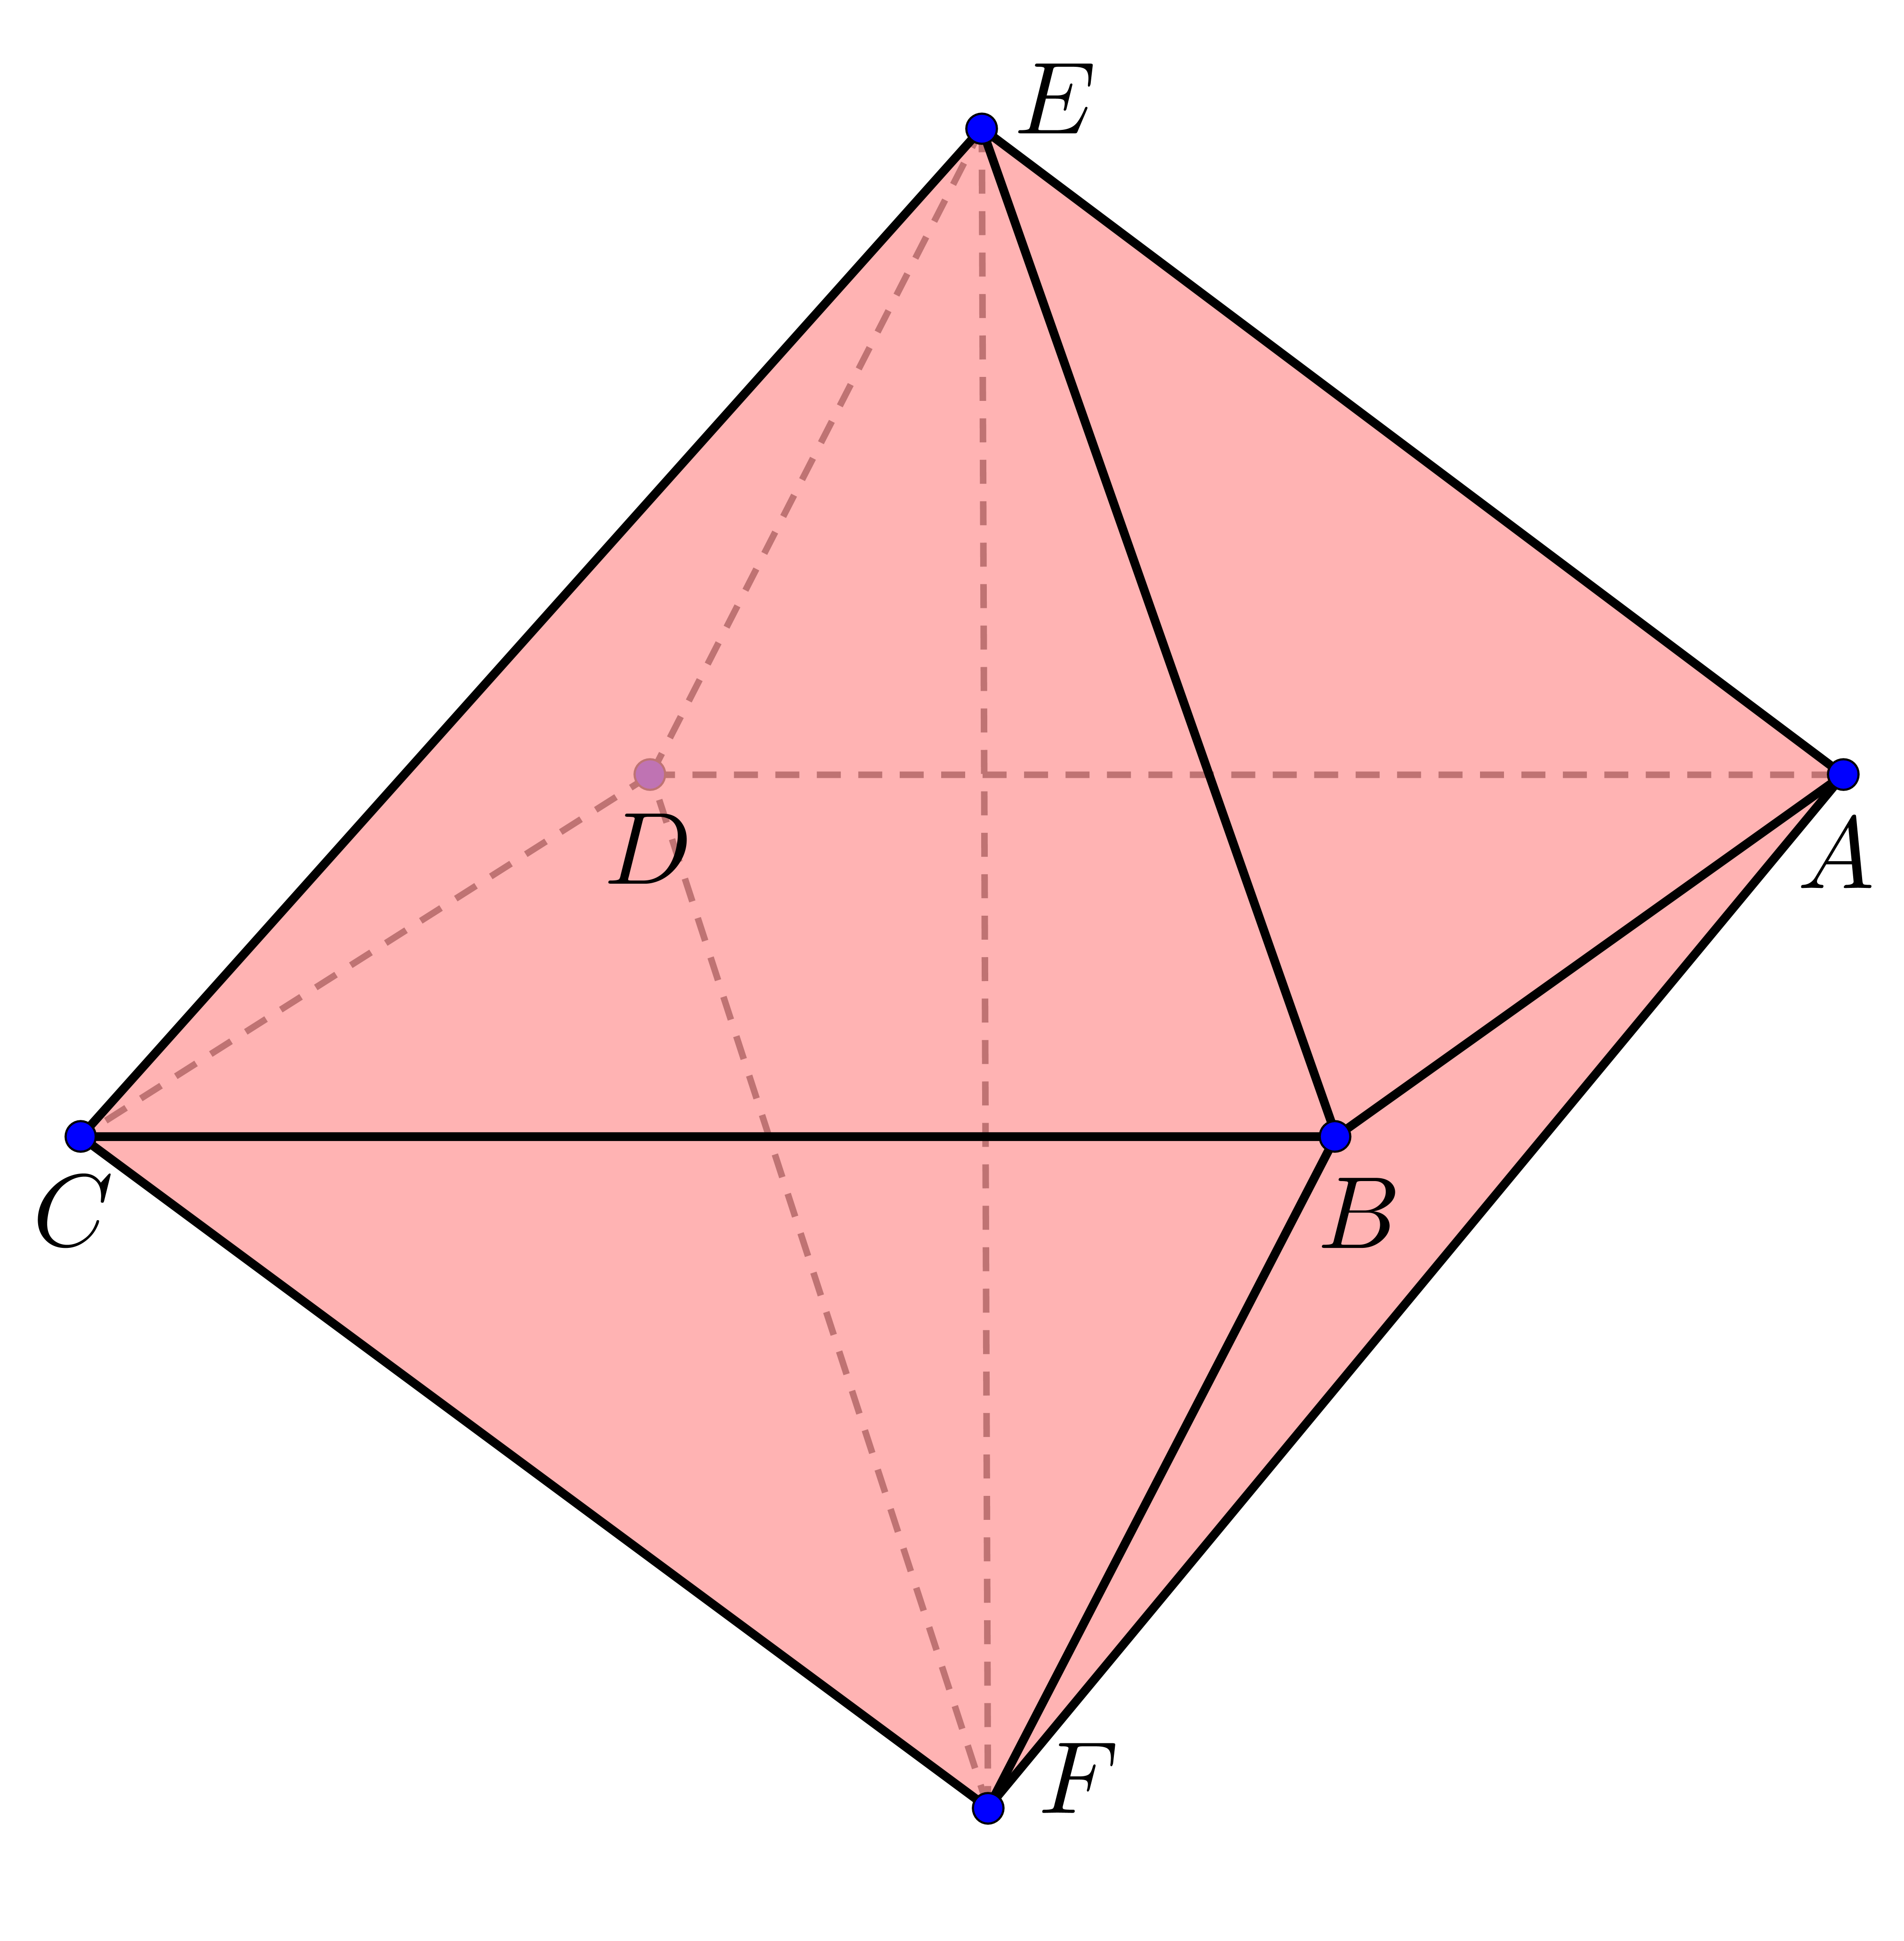
\includegraphics[width=0.5\linewidth]{./figures/octaedro.png}
\end{center}
\caption{Un octaedro bonito.}
\label{octaedro}
\end{figure}

Y puedes hacer referencia a la Figura \ref{octaedro}.

Puedes tambi\'en referenciar a otras etiquetas, por ejemplo, al Cap\'itulo \ref{Capitulo:TMD}.


